\subsection{INGRID Proton module}
INGRID Proton module is a neutrino detectors of the T2K experiment.
It is composed only with scintillator bars in its tracking region and surrounded by veto planes.. 
A different size scintillator bar was used to improve tracking capabilities. 
A schematic view of the Proton Module can be seen in Fig. \ref{fig:proton_module}. 


It was installed at the neutrino beam axis on the SS floor of the T2K near detector hall in 2010, and had been used for neutrino cross section measurements.
In August 2017, it was moved to the B2 floor of the same detector hall by J-PARC T59 after getting the approval from T2K to use them.
J-PARC T59 is performing neutrino beam measurement using the detector from October 2017, and the measurement  will continue until May 2018 as we will discuss in Sec. \ref{Sec:}.

\begin{figure}[tbh]
\begin{center}
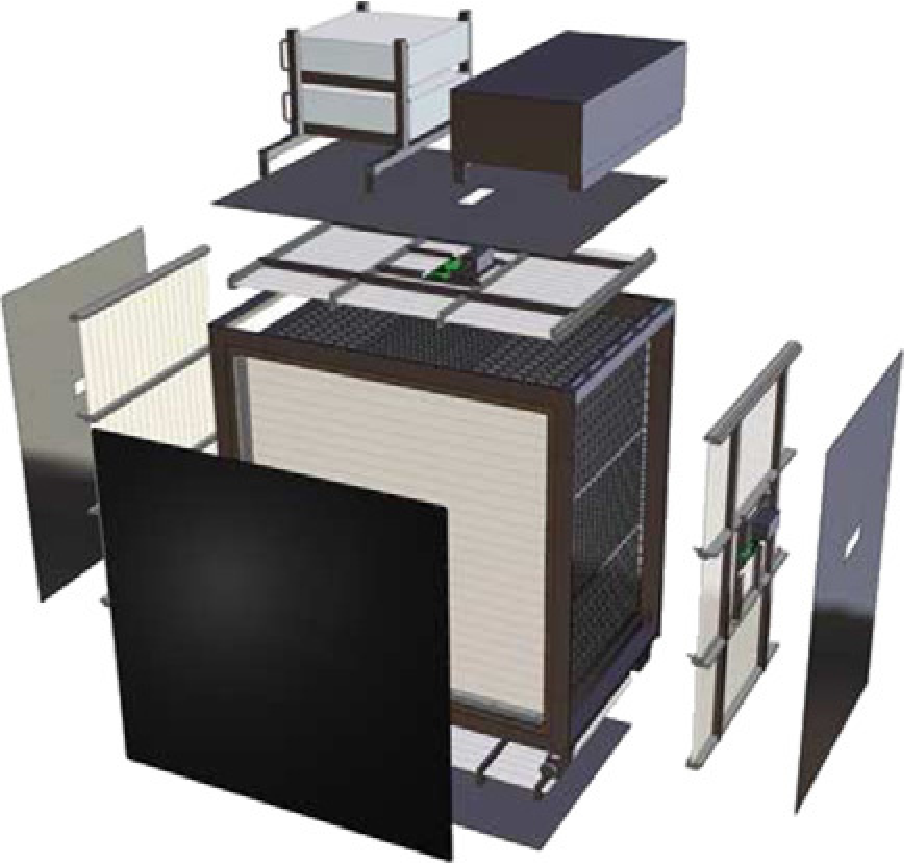
\includegraphics[width=0.6\linewidth]{fig/proton_module.pdf}
\end{center}
\caption{
Schematic view of INGRID Proton module.
}
\label{fig:proton_module}
\end{figure}
